
\documentclass{beamer}
\usepackage[latin1]{inputenc}
%\usetheme{Montpellier}
%\usetheme{Boadilla}
%\usecolortheme[RGB={204,51,255}]{structure}
%\usecolortheme[named=purple]{structure}
\usecolortheme[RGB={62,128,62}]{structure}
%\definecolor{reddish}{rgb}{0.3,0.15,0.3}
%\definecolor{light}{rgb}{0.8,0.6,0.8}
%\definecolor{reddish}{rgb}{.5,0.15,0.15}
\definecolor{reddish}{rgb}{0.5,0.3,0.4}
%\definecolor{light}{rgb}{0.8,0.6,0.8}
\definecolor{reddish}{rgb}{.7,0.25,0.25}
\definecolor{greenish}{rgb}{.25,0.7,0.25}
\definecolor{blueish}{rgb}{.25,0.25,0.7}
\definecolor{purple}{rgb}{.5,0.0,0.5}
\usepackage{graphicx}
\usepackage{pstricks}

\newcommand{\btVFill}{\vskip0pt plus 1filll}

\setbeamertemplate{navigation symbols}{}

\newcommand{\crish}{\color{reddish}}
\newcommand{\cbla}{\color{black}}
\newcommand{\cred}{\color{red}}
\newcommand{\cblu}{\color{blue}}
\newcommand{\cgre}{\color{green}}

\newcommand{\sm}{\color{reddish}$}
\newcommand{\fm}{$\color{black}{}}

\newcommand{\letter}[1]{\color{blue}\texttt{#1}\color{black}}
\newcommand{\binary}[1]{\color{red}\texttt{#1}\color{black}}

\usepackage{tikz}
\usetikzlibrary{arrows,decorations.markings,positioning}
\usepackage{epstopdf}
\usetikzlibrary{fit}

\title[Information Theory lecture 6]{Information in the brain: information theory lecture 6}
\author{COMSM0075 Information Processing and Brain}
\institute{\texttt{comsm0075.github.io}}
\date{October 2020}

\begin{document}

\maketitle


\begin{frame}{Neurons}
\color{reddish}
\begin{center}
\includegraphics[width=8cm]{PC.png}
\end{center}
\btVFill
\begin{flushright}
\tiny{Picture from wikisource.}
\end{flushright}
\end{frame}

\begin{frame}{Spikes}
\color{reddish}
\begin{center}
\includegraphics[width=8cm]{spike.png}
\end{center}
\btVFill
\begin{flushright}
\tiny{Picture from Hodgkin and Huxley, 1939.}
\end{flushright}
\end{frame}


\begin{frame}{Zebra finch}
\color{reddish}
\begin{center}
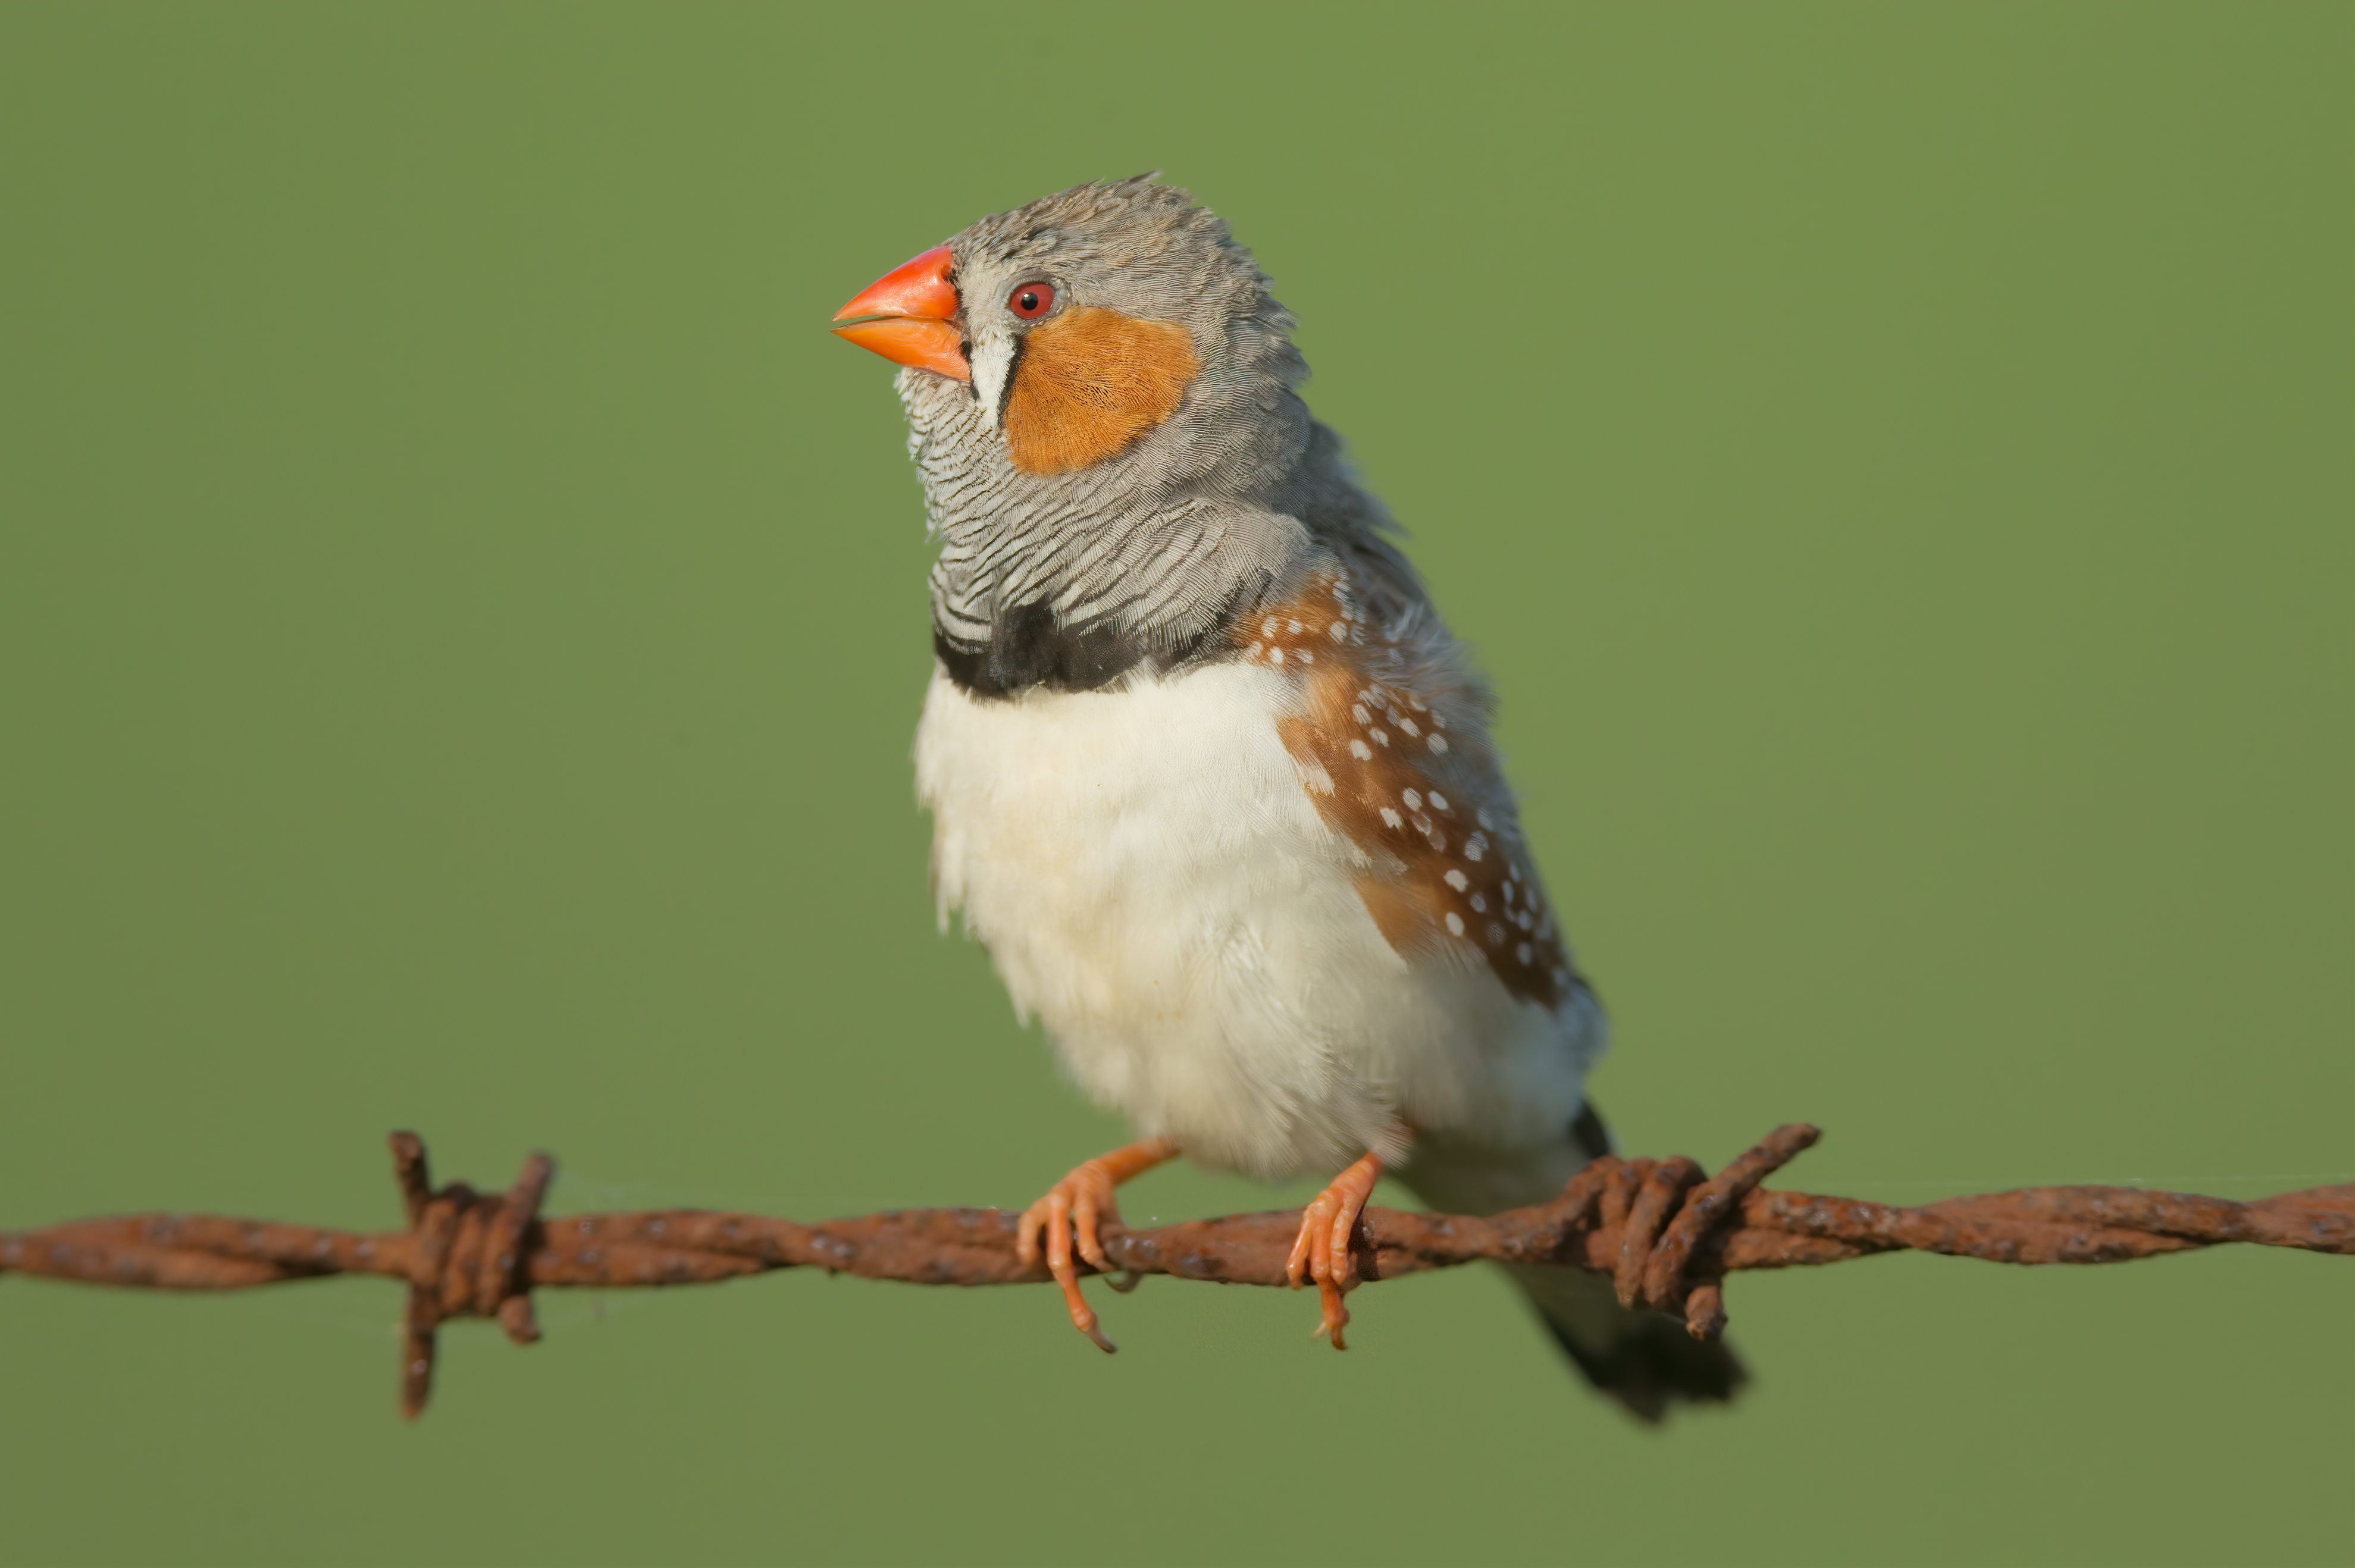
\includegraphics[width=8cm]{zebra_finch.jpg}
\end{center}
\btVFill
\begin{flushright}
\tiny{Picture from wikipedia.}
\end{flushright}
\end{frame}

\begin{frame}{Spike trains}
\color{reddish}
\begin{center}
\includegraphics[width=8cm]{SpikeTrains.png}
\end{center}
\end{frame}

\begin{frame}{Shannon's entropy}
\color{reddish}
$$
H(X)=-\sum_i p_X(x_i)\log_2{p_X(x_i)}
$$
\color{black}
\end{frame}

\begin{frame}{Fly}
  \begin{center}
    \includegraphics[width=8cm]{pence_fly.jpg}
  \end{center}
\end{frame}

\begin{frame}{Experiment by Bialek and coworkers}
  \begin{center}
    \includegraphics[width=8cm]{Blow-Fly.jpg}
  \end{center}
\end{frame}
  

\begin{frame}{Experiment by Bialek and coworkers}
  \begin{center}
    \includegraphics[width=8cm]{experiment1.jpg}
  \end{center}
\end{frame}
  

\begin{frame}{Experiment by Bialek and coworkers}
  \begin{center}
    \includegraphics[width=8cm]{experiment2.jpg}
  \end{center}
\end{frame}

\begin{frame}{Experiment by Bialek and coworkers}
  \begin{center}
    \includegraphics[width=8cm]{experiment3.jpg}
  \end{center}
\end{frame}

\begin{frame}{Experiment by Bialek and coworkers}
  \begin{center}
    \includegraphics[width=8cm]{experiment4.jpg}
  \end{center}
\end{frame}

\begin{frame}{Experiment by Bialek and coworkers}
  \begin{center}
    \includegraphics[width=8cm]{experiment7.jpg}
  \end{center}
\end{frame}

\begin{frame}{Experiment by Bialek and coworkers}
  \begin{center}
    \includegraphics[width=8cm]{experiment5.jpg}
  \end{center}
\end{frame}

\begin{frame}{Experiment by Bialek and coworkers}
  \begin{center}
    \includegraphics[width=8cm]{experiment6.jpg}
  \end{center}
\end{frame}

\begin{frame}{Experiment by Bialek and coworkers}
  \begin{center}
    \includegraphics[width=8cm]{experiment3.jpg}
  \end{center}
\end{frame}


\begin{frame}{Experiment by Bialek and coworkers}
  \begin{center}
    \includegraphics[width=8cm]{experiment7.jpg}
  \end{center}
\end{frame}

\begin{frame}{Discretize}
  \crish
  \begin{center}
\include{discretization}
  \end{center}
  \cbla
  \end{frame}

\begin{frame}{Split into words}
  \crish
  $$
  010001000000100\rightarrow 01000,10000,00100
  $$
  \cbla
\end{frame}


\begin{frame}{$W$}
  \crish
  \begin{eqnarray*}
\textbf{w}_0&=&(0,0,0,0,0)\cr
\textbf{w}_1&=&(0,0,0,0,1)\cr
\textbf{w}_2&=&(0,0,0,1,0)\cr
\textbf{w}_3&=&(0,0,0,1,1)\cr
&&\ldots
\end{eqnarray*}
  \cbla
\end{frame}


\begin{frame}{$W$}
  \crish
  \begin{eqnarray*}
\textbf{w}_0&=&(0,0,0,0,0)\cr
\textbf{w}_1&=&(0,0,0,0,1)\cr
\textbf{w}_2&=&(0,0,0,1,0)\cr
\textbf{w}_3&=&(0,0,0,1,1)\cr
&&\ldots
\end{eqnarray*}
  \cbla
  and
  \crish
  $$p(\mathbf{w}_0)\approx\frac{\#(\mbox{occurance of }\mathbf{w}_0)}{\#(\mbox{trials})}$$
  \cbla
\end{frame}



\begin{frame}{$H(W)$}
  
  $$
  01000,10000,00100,10000,01000,01100,00011,00110,01000,\ldots
  $$
  
  \end{frame}


\begin{frame}{$H(W|S)$}
  \begin{tabular}{ccccc}
   $s_1$&$s_2$&$s_3$&$s_4$&$\ldots$\\  
   01000&10000&00100&10100&$\ldots$\\
   00100&11000&00001&01000&$\ldots$\\
   01010&00000&00100&00010&$\ldots$\\
   01000&01000&10100&10010&$\ldots$\\
   01100&10010&01100&00100&$\ldots$
  \end{tabular}
\end{frame}

\begin{frame}{$H(W|S)$}
  \begin{tabular}{ccccc}
   $s_1$&$s_2$&$s_3$&$s_4$&$\ldots$\\  
   01000&\cblu{}10000\cbla{}&00100&10100&$\ldots$\\
   00100&\cblu{}11000\cbla{}&00001&01000&$\ldots$\\
   01010&\cblu{}00000\cbla{}&00100&00010&$\ldots$\\
   01000&\cblu{}11000\cbla{}&10100&10010&$\ldots$\\
   01100&\cblu{}10010\cbla{}&01100&00100&$\ldots$
  \end{tabular}
  \cblu
  $$
  p(W=11000|S=s_2)\approx\frac{\#(11000)}{\#(\mbox{trials})}=\frac{2}{5}
  $$
  \cbla
\end{frame}


\begin{frame}{$I(W,S)$}
  \crish
  $$I(W,S)=H(W)-H(W|S)$$
  \cbla
  or
  \begin{center}
    information about \crish$S$\cbla{} in \crish$W$\cbla= total information  in \crish$W$\cbla - noise
  \end{center}
\end{frame}

\begin{frame}{discretization size}
  \begin{quote}
One question is how to decide how small to make the discretization time and how long to make the words. It is argued that the blowfly responds very quickly to attempts to swat it, so the information coming from H1 is being interpreted by other brain areas over a time scale of 30 ms.
  \end{quote}
\end{frame}


\begin{frame}{result}
\vskip 2cm
\cblu $\delta t=3$ ms\cbla{} gives \cblu $78\pm 5$ bits per second \cbla or \cblu $1.8\pm 0.1$ bits per spike\cbla. 
\btVFill
\begin{flushright}
\tiny{Strong et al. 1998}
\end{flushright}
\end{frame}


\begin{frame}{too many words}
  30 ms words with 3 ms letters:
  \crish
  $$
  2^{10}=1024
  $$ \cbla
\end{frame}


\begin{frame}{too many words}
  30 ms words with 3 ms letters:
  \crish
  $$
  2^{10}=1024
  $$ \cbla
  \begin{quote}
  If six seconds of data are used for the repeating stimulus, that is 100 different stimuli, then even for a three hour recording, there are 1800 trails for each stimulus, not a huge amount for estimating 1024 probabilities.
  \end{quote}
\end{frame}


\end{document}

